\chapter{Aeroelastic study} \label{chap:aeroelastic}

  %Intro
  In the present chapter, the compliant design for the wing-box is embedded into a full wing model. A pressure field is then introduced to simulated the pressure distribution obtained from the evaluation of the aerodynamic forces around the airfoil.

  \section{Wing model} \label{sec:wingModel_aeroelastic}

    The wing is modeled in its half span dimension and the airfoil is one symmetric NACA 0012. An overview of the wing model can be seen in Figure \ref{fig:wing}.

    \begin{figure}[!htpb]
      \centering
      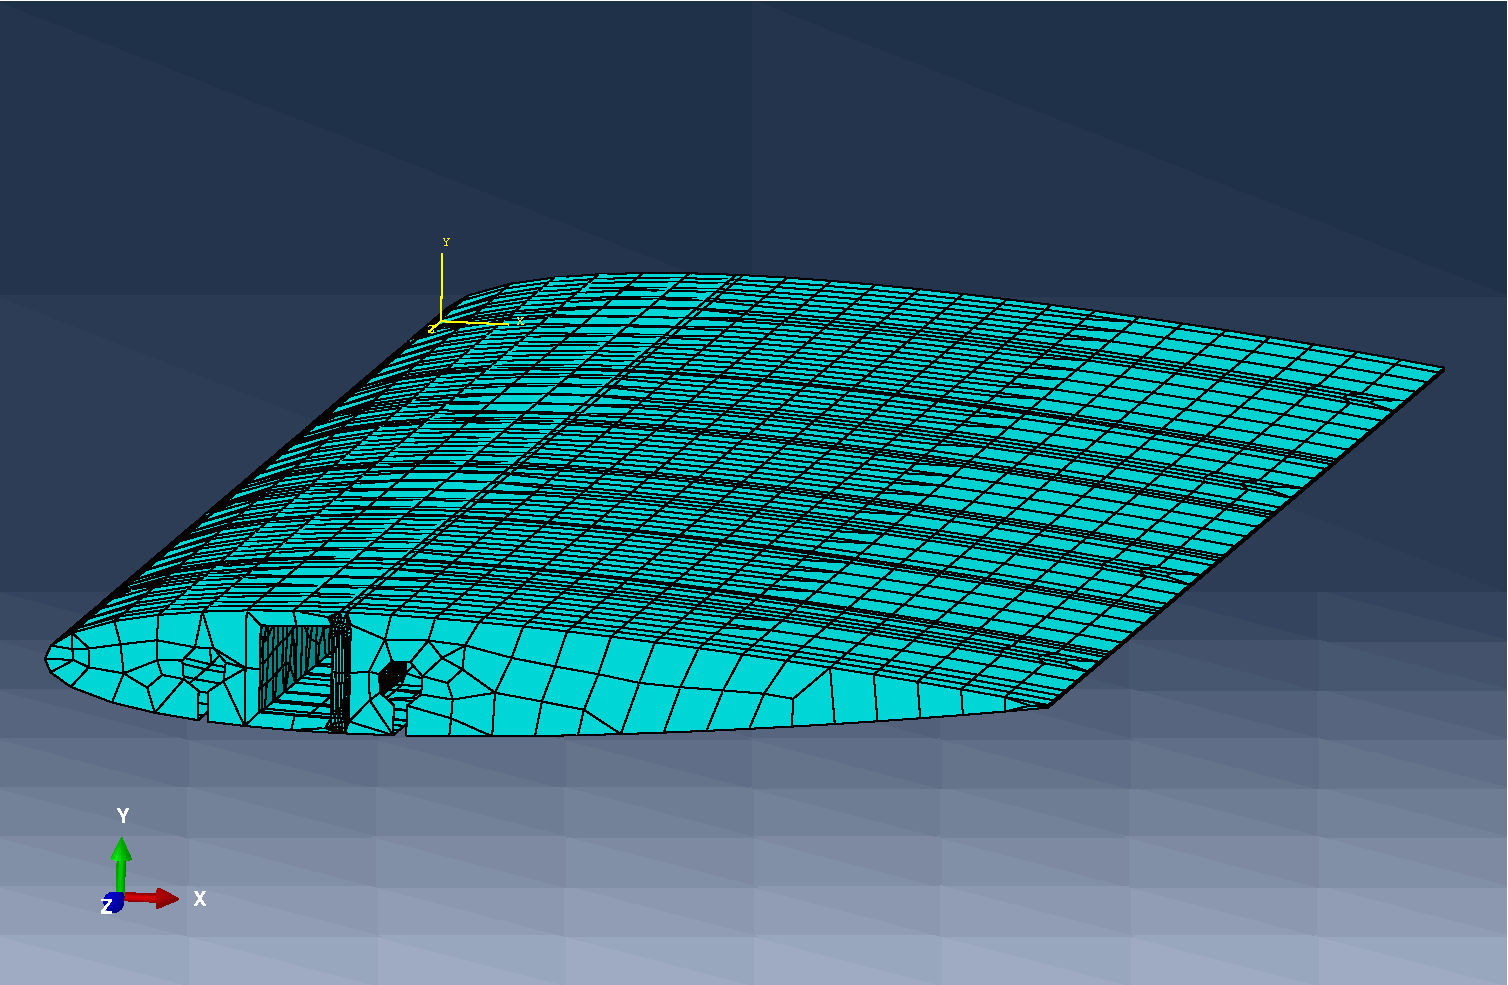
\includegraphics[width=0.8 \textwidth]{figures/wing-model/wing}
      \caption[Overview of the wing FEM model embedded with the compliant wing-box design]{Overview of the wing FEM model embedded with the compliant wing-box design.}
      \label{fig:wing}
    \end{figure}
    
    The boundary condition for the wing-box includes establish a free condition at the tip of the wing and a clamping condition at the root.

  \section{Aerodynamic forces} \label{sec:aerodynamic_aeroelastic}

    The pressure distribution originated from the fluid-airfoil interaction is modeled and it is responsible of the forces applied into the wing model. This is the only source of forces introduced into the model.